\begin{customAppendixPage}{Work Distribution}
This appendix contains the operating charts for the different event services that compose the system.  A brief explanation of each chart is included.
\end{customAppendixPage}
\renewcommand*{\thepage}{\thesection-\arabic{page}}

\subsection{Diagnostic Event Service}

In this service, called Diagnostic Mode, the device maintains communication to the base station and sends real-time measurement information of the different components to the base station. The user can then observe and verify that all components are taking accurate measurements and that data can be retrieved through the XBee module. If the user decides to exit Diagnostic mode, he will do so by choosing the option at the base station, which will send the corresponding signal to the Xbee module and interrupt the MCU. The Diagnostic flag will be cleared by the interrupt routine, and will cause the return of the Diagnostic Event Service, shown below.


\begin{figure}[H]
	\centering
	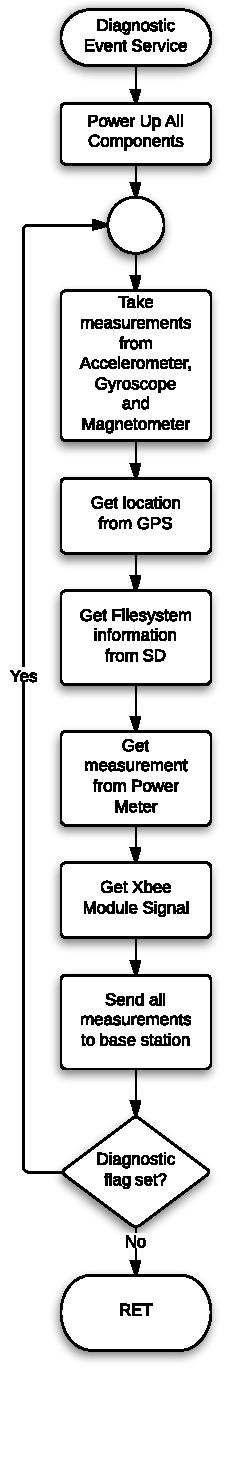
\includegraphics[scale=0.7]{img/DiagnosticEventService}
	\caption{Flowchart for Diagnostic Event Service \label{fig:diagnosticMode}}
\end{figure}

\subsection{Sampling Event Service}
While in Sampling Mode, the device captures data from the accelerometer, gyroscope and magnetometer. Data is captured for 30 seconds and data points are saved in the SD card, each with a time stamp from the time when they were captured.
\begin{figure}[H]
	\centering
	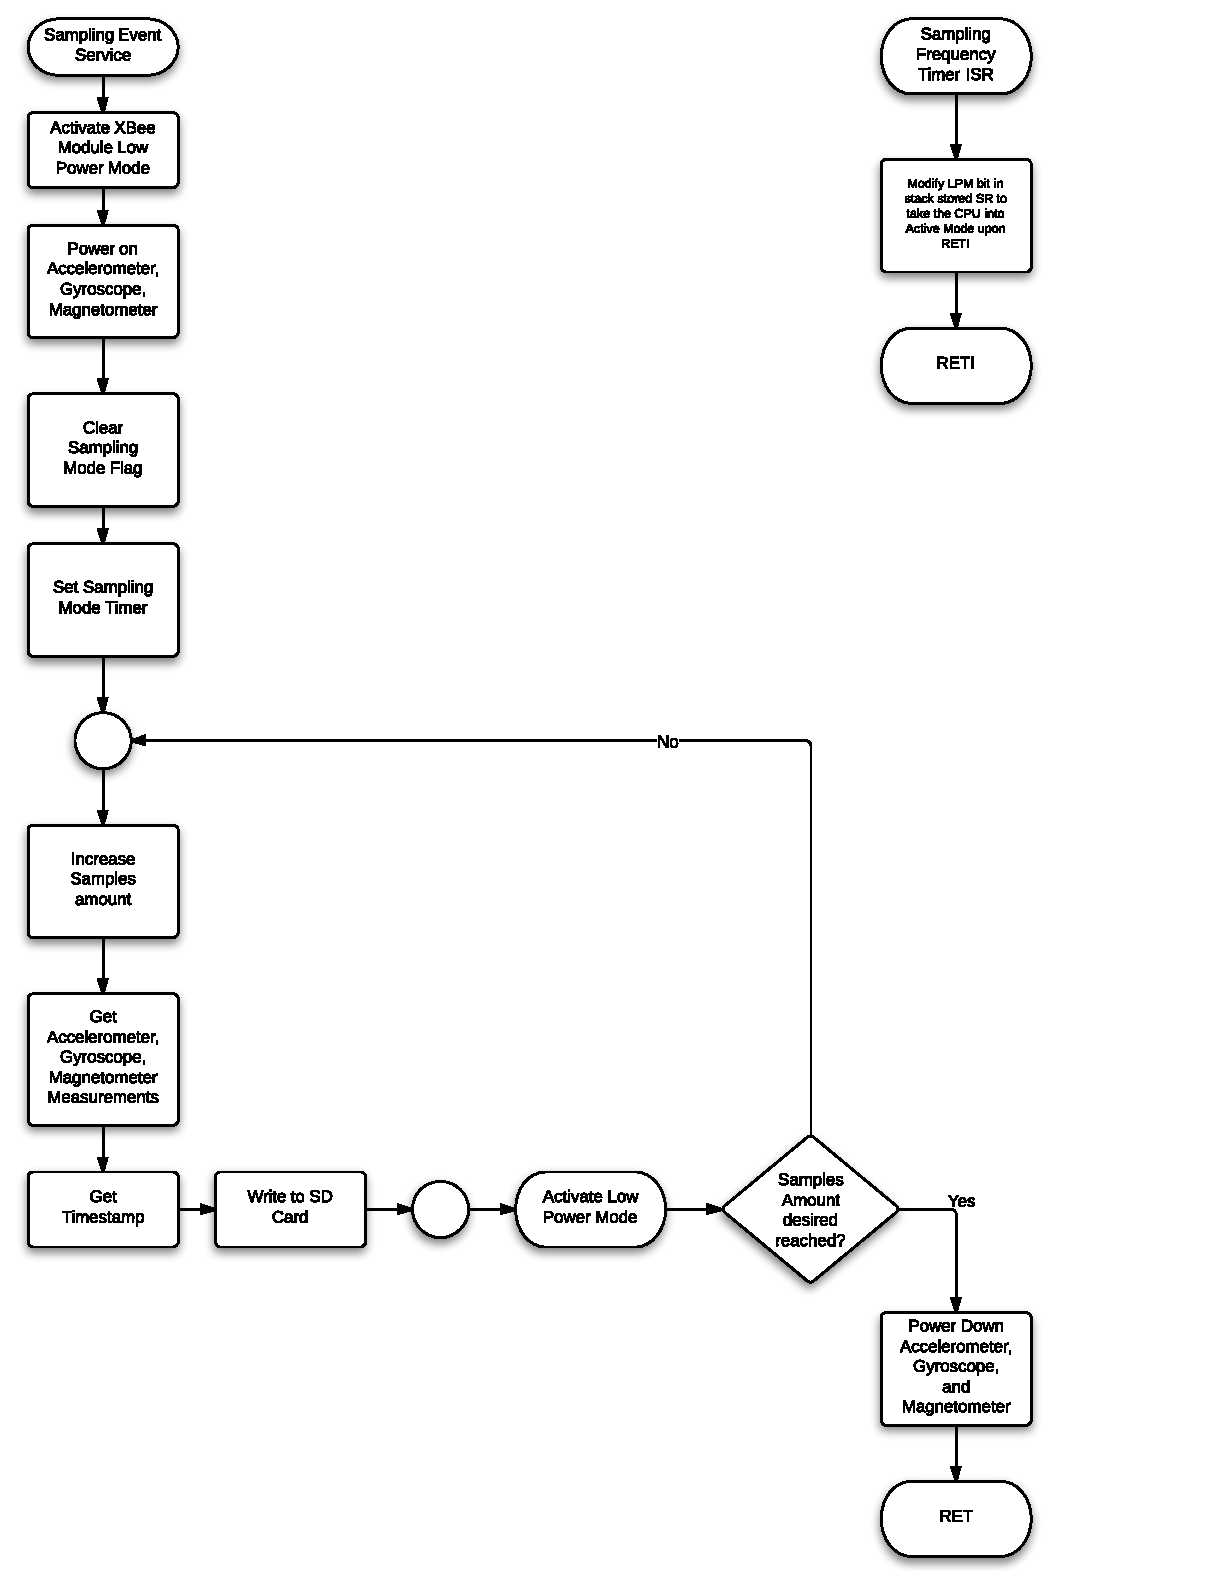
\includegraphics[scale=0.7]{img/SamplingEventService}
	\caption{Flowchart for Sampling Event Service \label{fig:samplingMode}}
\end{figure}

\subsection{Retrieval Event Service}
Retrieval Mode is the operation mode of the device in which the system transfers the data collected while it was in Sampling Mode. This mode transfers the data from the SD Card to the base station. Data is transferred trough the established ZigBee connection and once all data has been transferred it is erased from the SD card.
\begin{figure}[H]
	\centering
	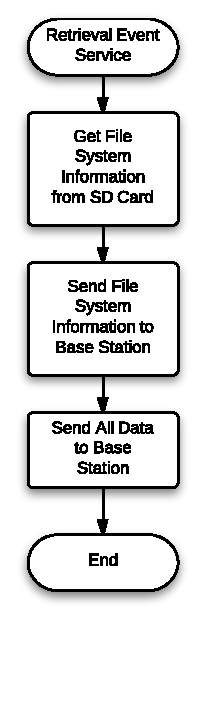
\includegraphics[scale=1.0]{img/RetrievalEventService}
	\caption{Flowchart for Retrieval Event Service \label{fig:retrivalMode}}
\end{figure}

\subsection{Location Event Service}
While in Locate Mode, the user is trying find and retrieve the device. The system turns on the XBee Module and the GPS. The system then proceeds to establishing a ZigBee connection to the base station and get a GPS lock. Once the device gets its location using the GPS Module it will then broadcast the location to the base station through the ZigBee connection.
\begin{figure}[H]
	\centering
	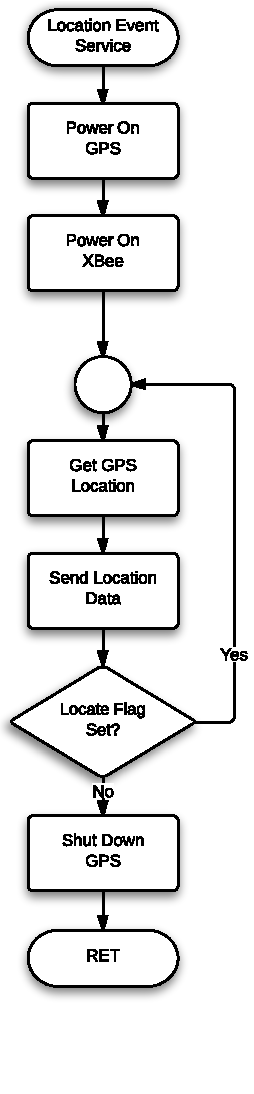
\includegraphics[scale=0.8]{img/LocationEventService}
	\caption{Flowchart for Location Event Service \label{fig:locateMode}}
\end{figure}

\subsection{Status Event Service}
The status event service will send battery charge status and SD card information to the base station. The SD card information includes free space and file system information.
\begin{figure}[H]
	\centering
	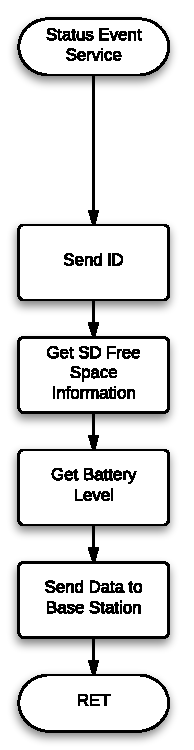
\includegraphics[scale=0.8]{img/StatusEventService}
	\caption{Flowchart for Status Event Service \label{fig:statusMode}}
\end{figure}